%--------------------------------------------------------------------
\section{Introduction}

RDF (Resource Description Framework) is designed to facilitate machine interpretability of information and does not define a visual presentation model since human readability is not one of its stated goals. Displaying RDF data in a user-friendly manner is a problem addressed by various types of applications using different representation paradigms. Web-based tools such as Longwell \cite{simile} (see Figure \ref{rdfBrowsers}-a) and Piggy-Bank \cite{huynh05} use nested box layouts, or table-like layouts (e.g. Brownsauce \cite{Steer03}, Noadster \cite{Rutledge05}, Swoop \cite{MindSwap05}) for displaying properties of RDF resources with varying levels of details. Other tools like IsaViz \cite{isaviz} (see Figure \ref{rdfBrowsers}-b) and Welkin \cite{Welkin} represent RDF models as node-link diagrams, explicitly showing their graph structure. A third approach combines these paradigms and extends them with specialized user interface widgets designed for specific information items like calendar data, tree structures, or even DNA sequences, providing advanced navigation tools and other interaction capabilities: Haystack \cite{Quan03} (see Figure \ref{rdfBrowsers}-c), mSpace \cite{mspace2005} and Tabulator \cite{timbl06}.

\begin{figure}
\begin{center}
\begin{tabular}{ccc}
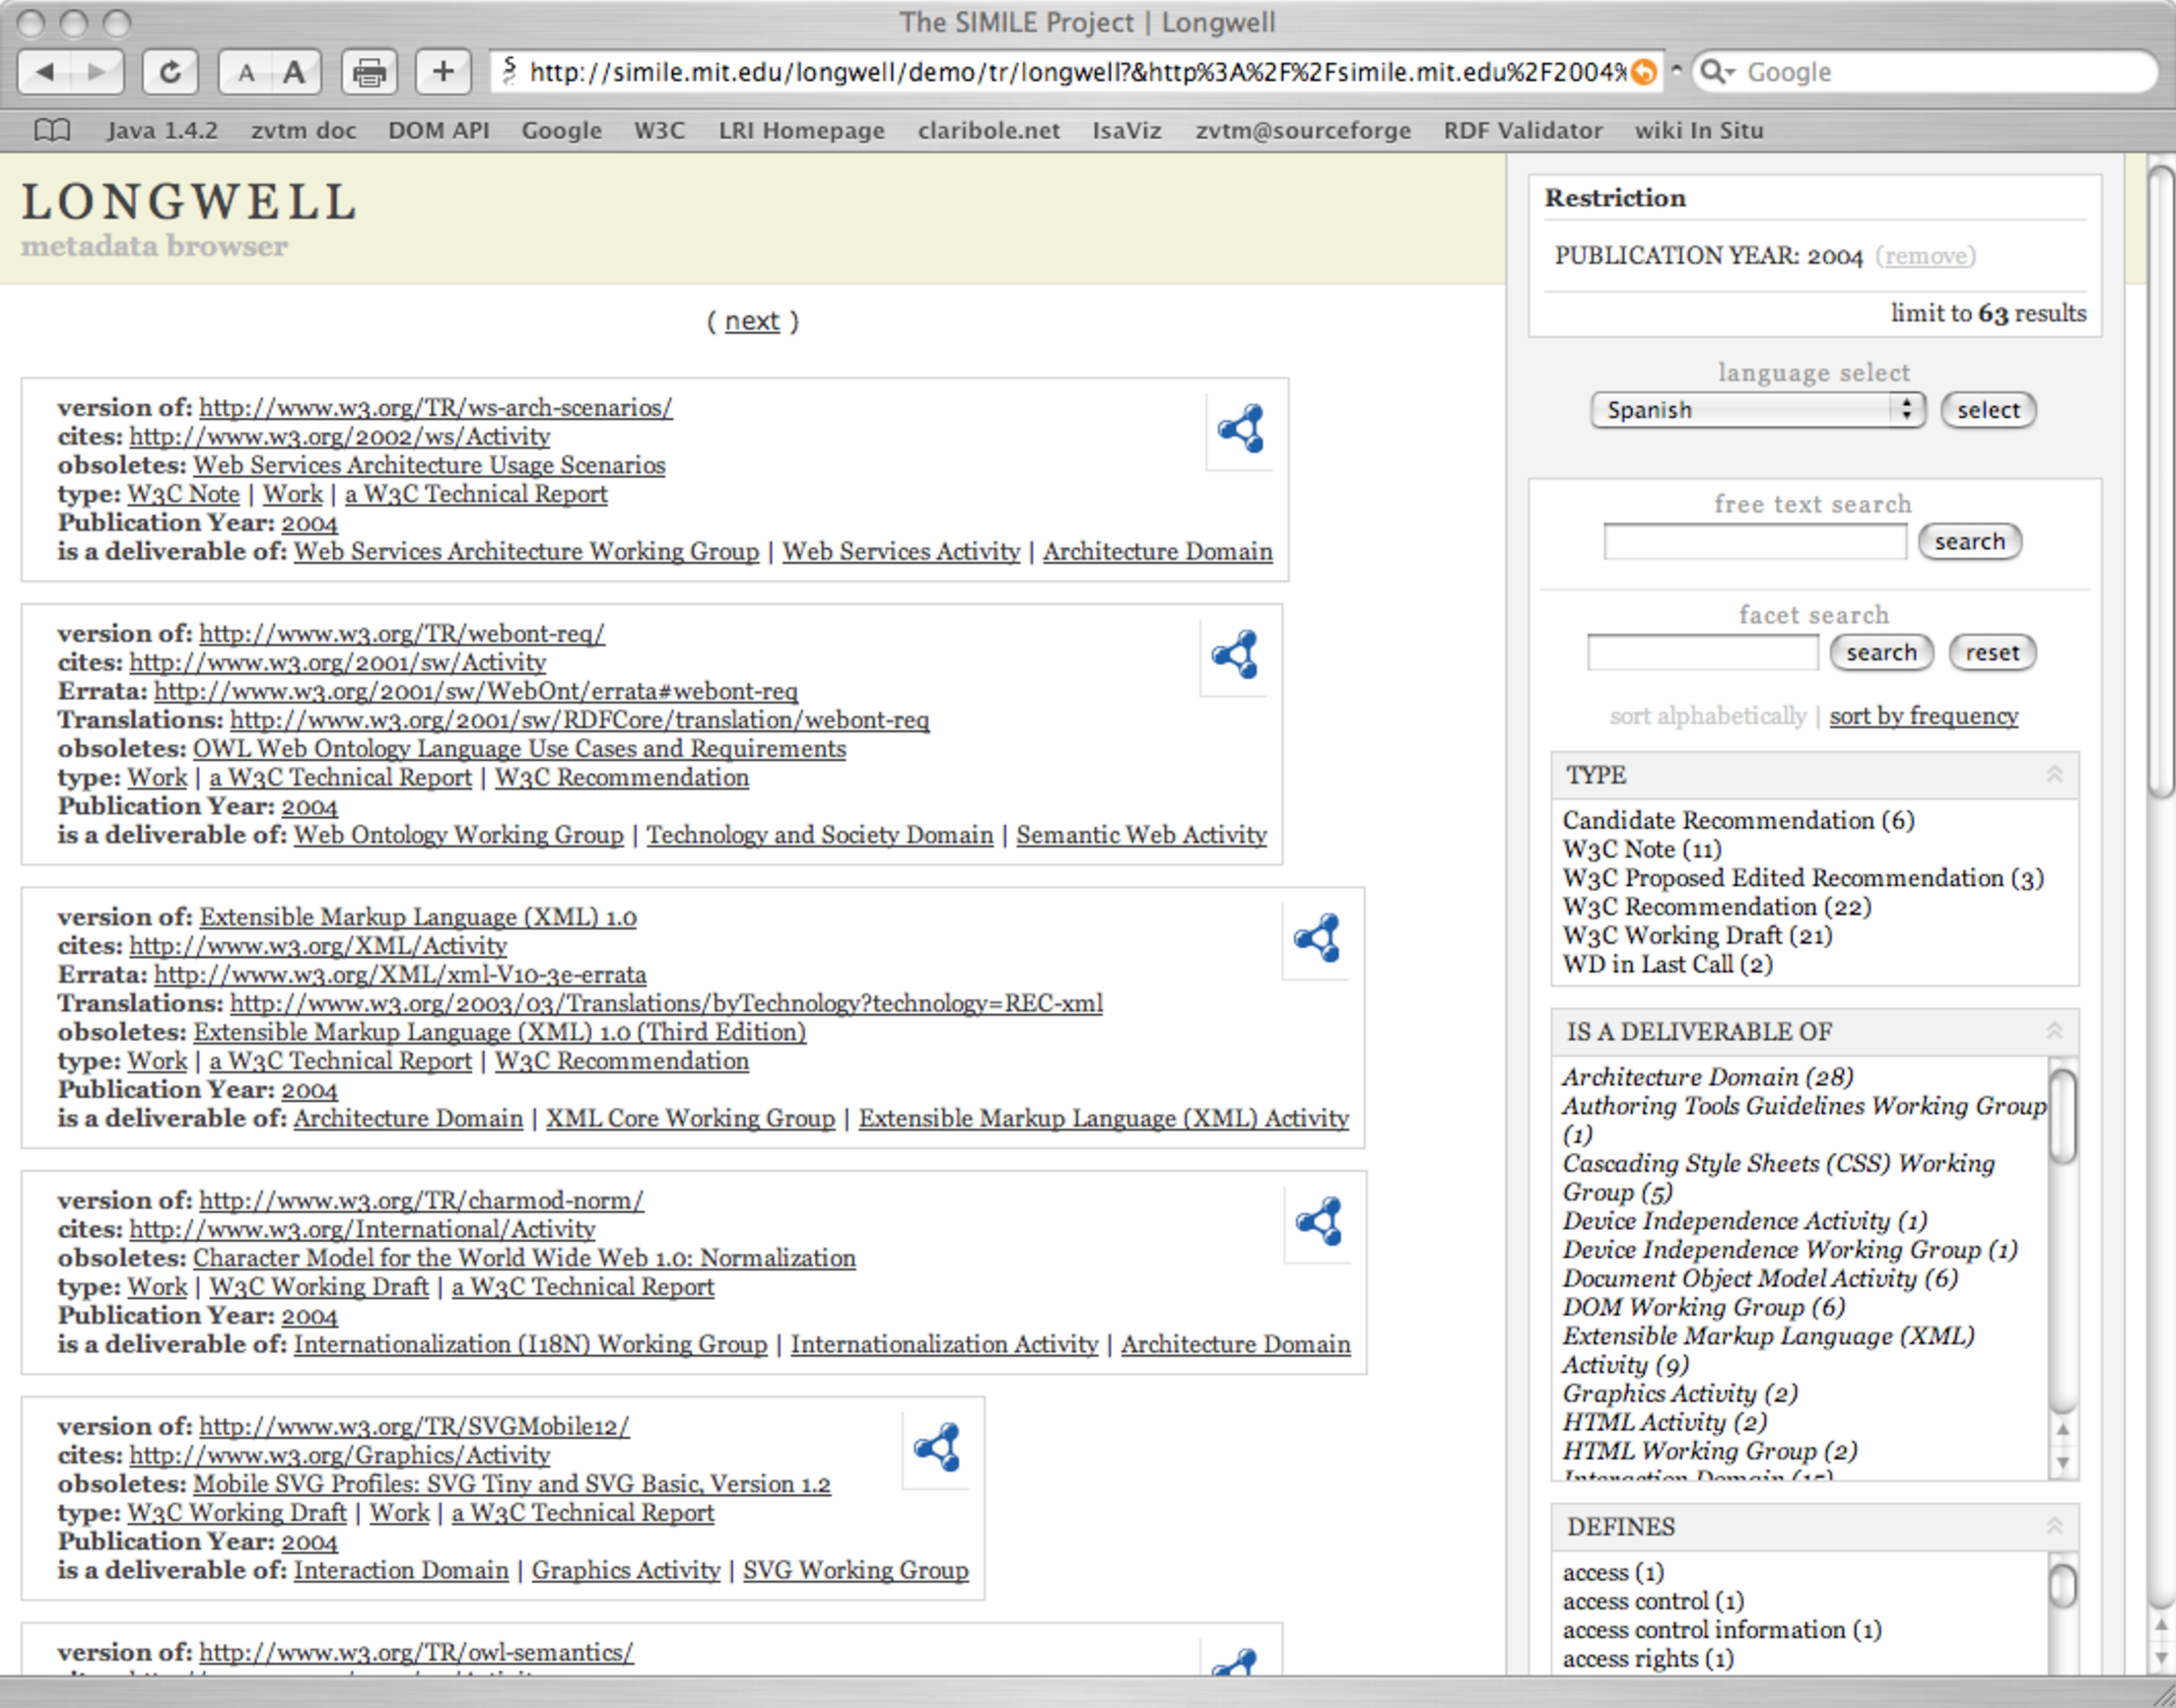
\includegraphics[height=3cm]{longwell.pdf} &
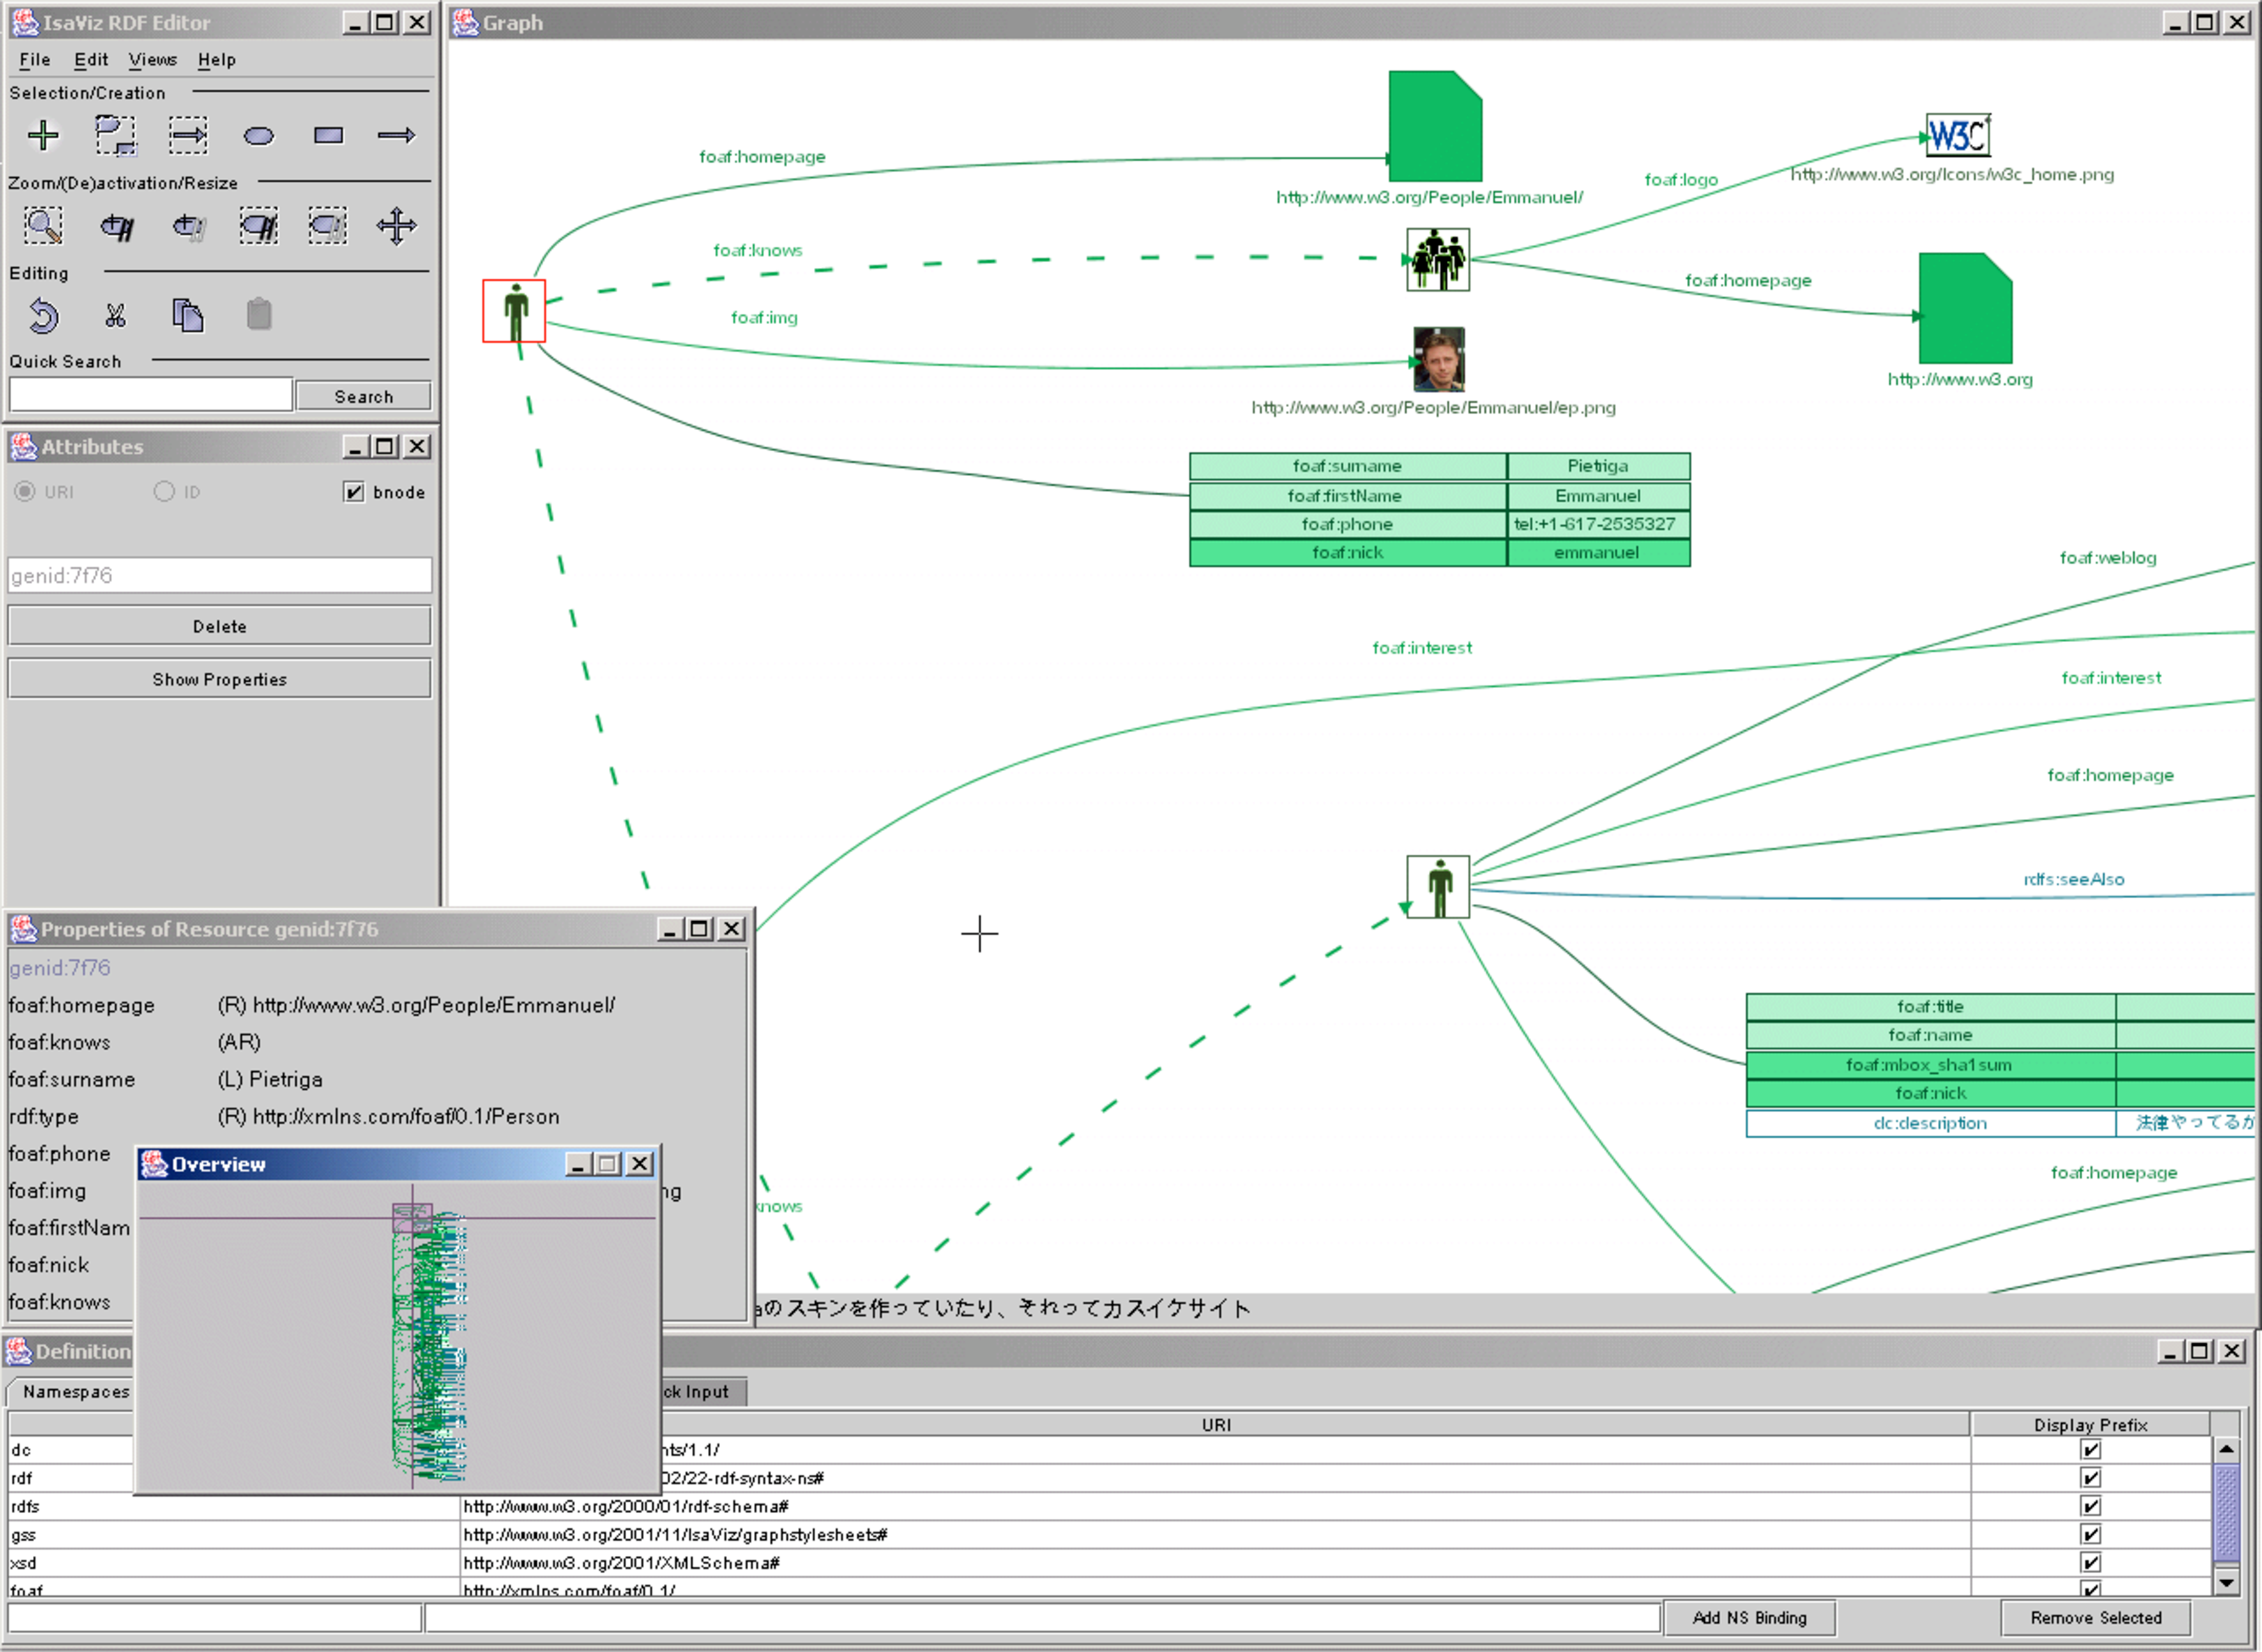
\includegraphics[height=3cm]{isaviz.pdf} &
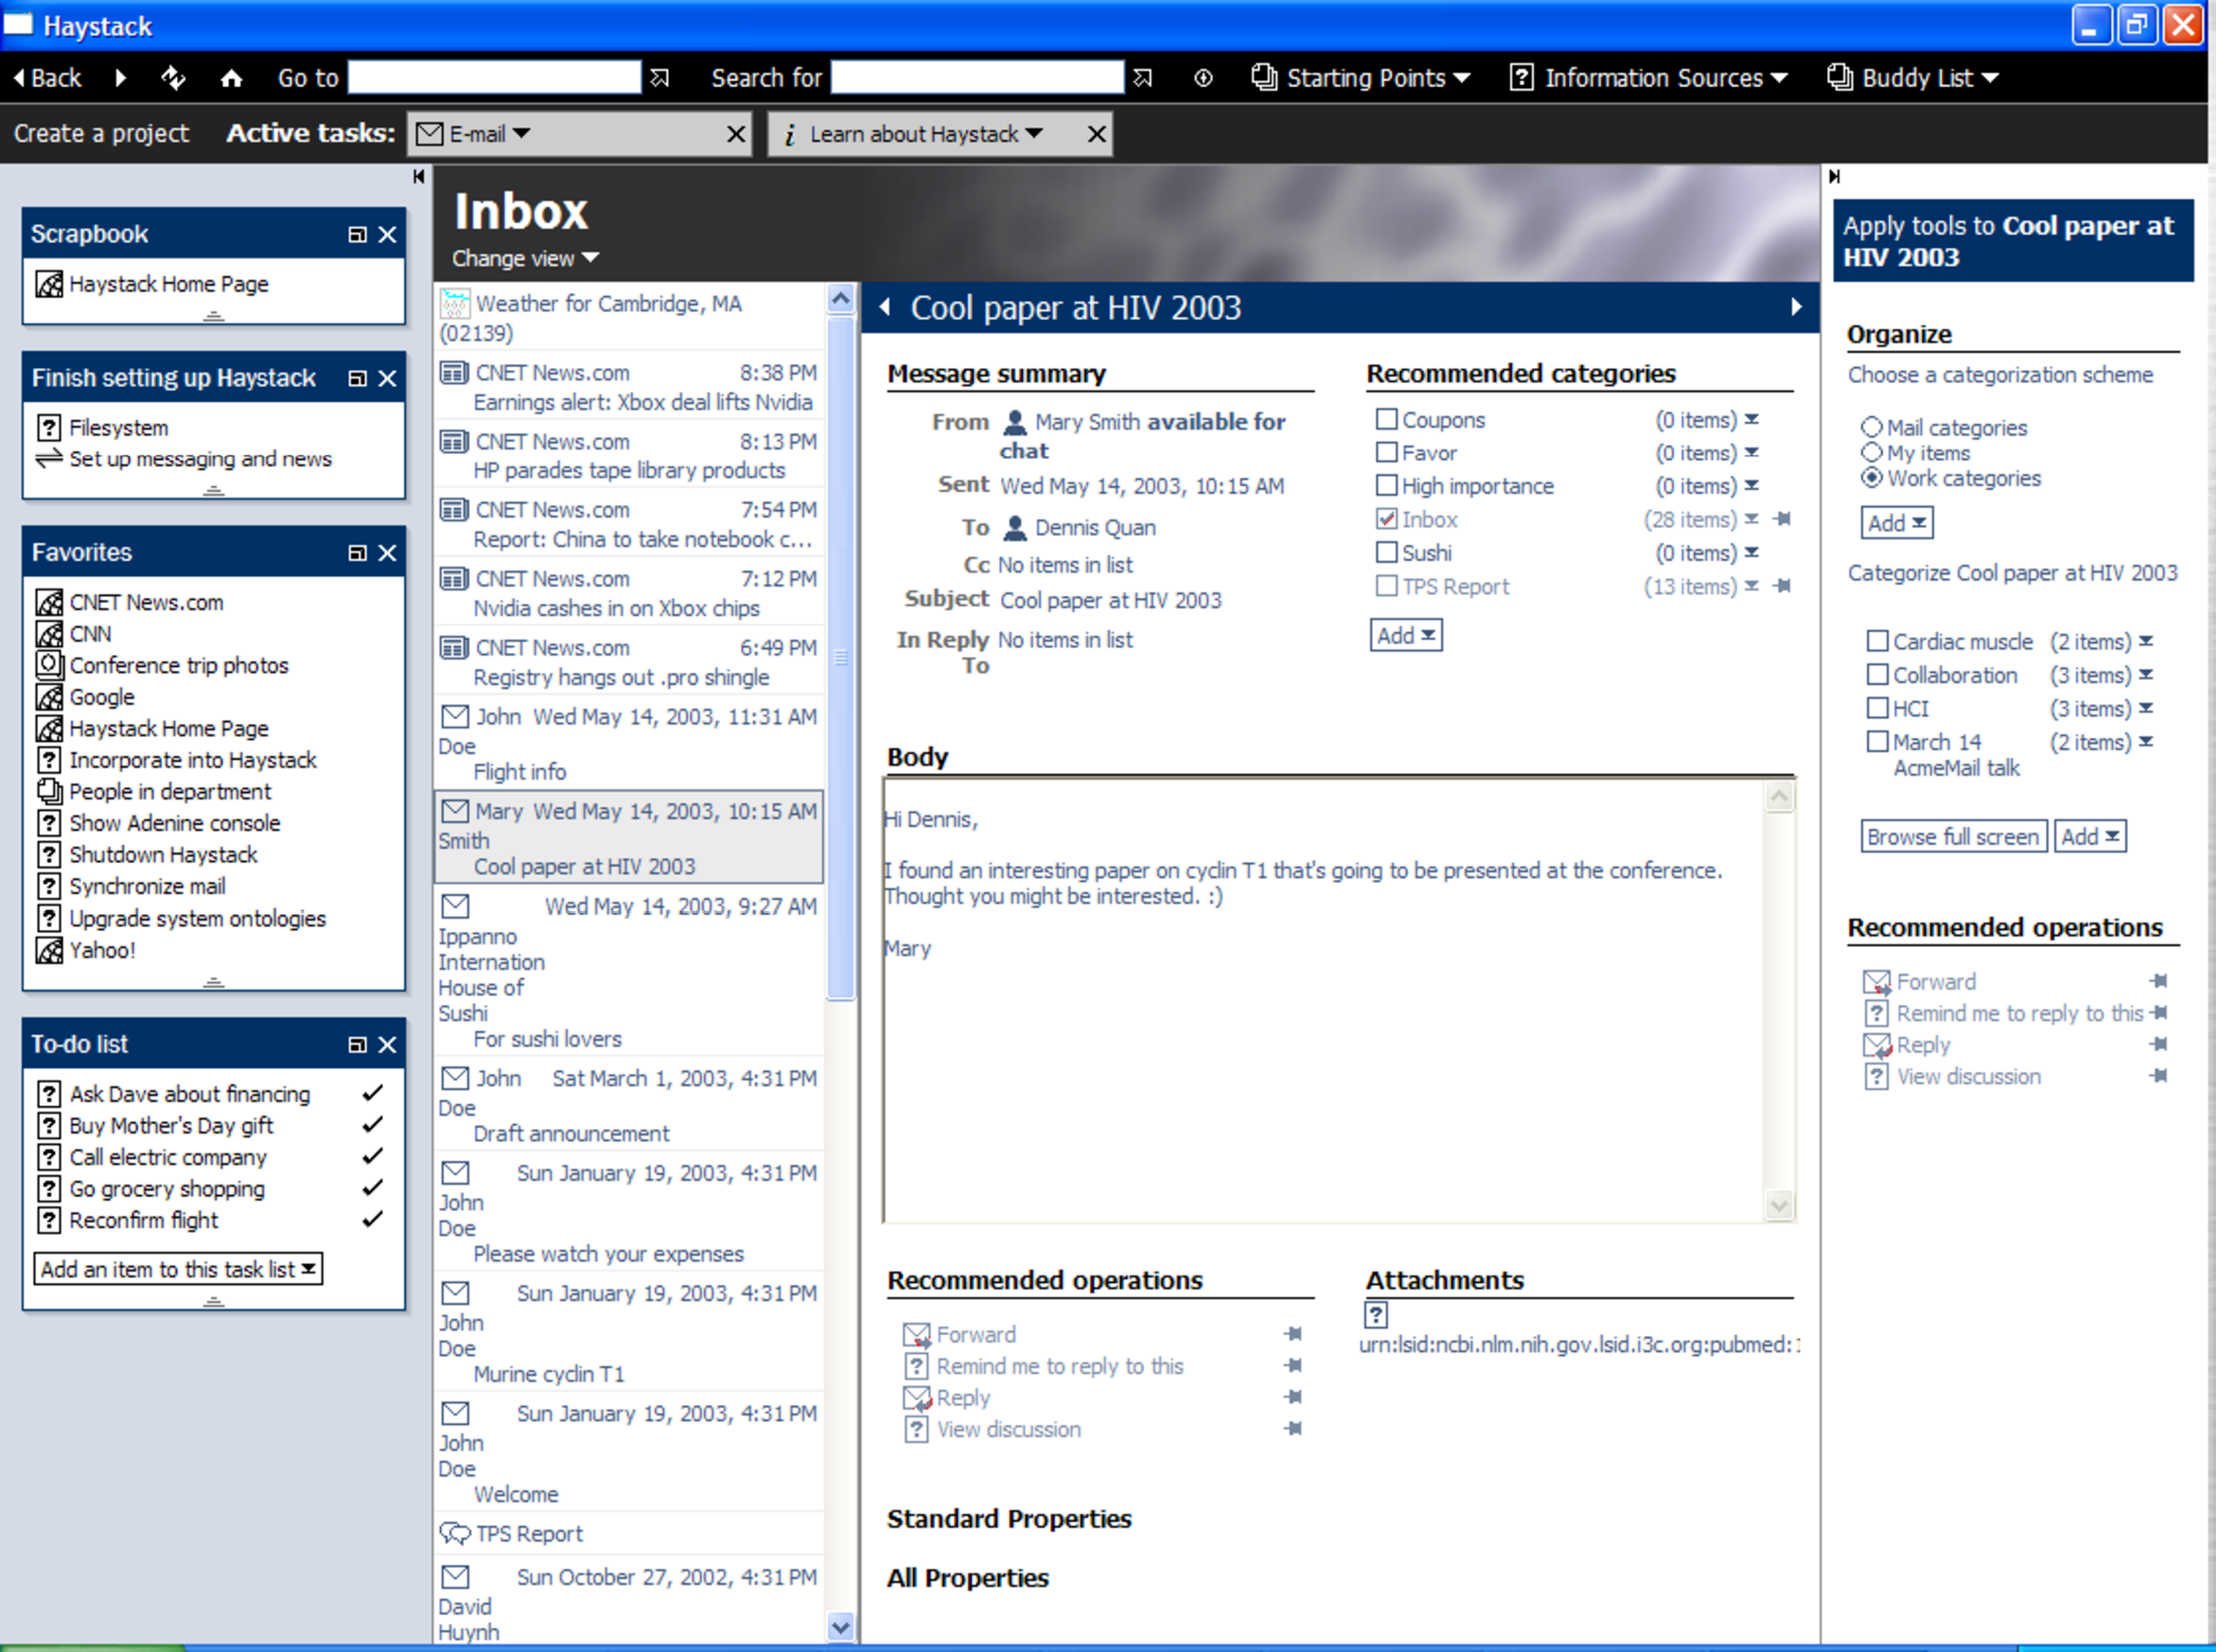
\includegraphics[height=3cm]{haystack.pdf} \\
(a) & (b) & (c)\\
\end{tabular}
\caption{Various types of RDF browsers: Longwell, IsaViz and Haystack}
\label{rdfBrowsers}
\end{center}
\end{figure}

Such applications are confronted with the same two issues, independently of the underlying representation paradigm and interface capabilities: selecting what content to show and specifying how to format and style this content. Each application takes its own approach and defines its own vocabulary to specify how to present data to users. As with other kinds of knowledge, we believe that being able to share what we consider {\em presentation knowledge} makes sense in the context of the Semantic Web and that being able to exchange and reuse presentation knowledge between browsers and other visualization tools will benefit both programmers and end users. However, the current diversity of approaches and vocabularies for representing this knowledge makes such exchange and reuse difficult at best, if not impossible.

\subsection{Related Work}

Early RDF visualization tools rendered RDF models in a predefined, non-custo\-mizable way \cite{Steer03}. Recent tools provide more flexible visualizations that can be customized by writing style sheets, transformations, or templates, following either a declarative or a procedural approach.

Procedural approaches consider the presentation process as a series of transformation steps. One such approach consists in using XSLT to transform RDF graphs encoded as RDF/XML trees in an environment such as Cocoon \cite{cocoon05}. Authoring XSLT templates and XPath expressions to handle arbitrary RDF/XML is complex, if not impossible, considering the many potential serializations of a given RDF graph and the present lack of a commonly accepted RDF canonicalization in XML \cite{Carroll04}. This problem has been partly addressed by Xenon \cite{quan05}, an RDF style sheet ontology that builds on the ideas of XSLT but combines a recursive template mechanism with SPARQL as an RDF-specific selector language. Xenon succeeds in addressing XSLT's RDF canonicalization problem but still has a drawback common to all procedural approaches, that transformation rules are tied to a specific display paradigm and output format, thus preventing the reuse of presentation knowledge across applications.

Declarative approaches are based on formatting and styling rules applied to a generic representation of the content. They can be compared to XHTML+CSS, which has been successful for the classic Web. The Haystack Slide ontology \cite{HaystackUI03}, used to describe how Haystack display widgets are laid out, is one example. Another is IsaViz's Graph Style Sheets \cite{pietriga06b}, which modifies the formatting, styling, and visibility of RDF graph elements represented as node-link diagrams. The main drawback of the declarative approaches developed so far is that they make strong assumptions about, and are thus tied to, the specific display paradigm for which they have been developed and are therefore unlikely to be meaningful across different representation paradigms.

\subsection{Toward the specification of presentation knowledge}

Providing a single global view of all the information contained in an
RDF model is often not useful. The mass of data makes it difficult to
extract information relevant to the current task and represents a
significant cognitive overload for the user. From an abstract
perspective, the first step of the presentation process thus consists
in restricting the visualization to small but cohesive parts of the
RDF graph, similarly to views in the database world. But identifying
what content to show is not sufficient
for making a human-friendly presentation from the information. To
achieve this goal, the selected content items must be laid out
properly and rendered with graphical attributes that favor legibility
in order to facilitate general understanding of the displayed
information. Relying solely on the content's structure and exploiting
knowledge contained in the schema associated with the data is
insufficient for producing sophisticated presentations and
visualizations. The second step thus consists in formatting and
styling selected content items.

Fresnel's goal is to provide an RDF vocabulary to encode information about how to present Semantic Web content to users (i.e., {\em what } content to show, and {\em how} to show it) as presentation knowledge that can be exchanged and reused between browsers and other visualization tools. However, we do not expect all applications, which do not necessarily rely on the same representation paradigms and formats, to exchange and reuse all formatting and styling instructions as some might not be appropriate for all paradigms. We therefore identified a set of core presentation concepts that are applicable across applications and which form the core modules of Fresnel. One of the design goals of these modules was to make them easy to learn and use, but also easy to implement in order to promote their adoption by many applications. On top of these modules, we have also begun to define additional Fresnel vocabulary items which are grouped in extension modules. The remainder of this article mainly focuses on the core selection and formatting modules. More information about extension modules can be found in the Fresnel User Manual \cite{fresnel05}.


